\chapter{Studi Literatur}

Pada bab ini, Penulis akan menguraikan hasil literatur dalam penyusunan tugas
akhir ini. Subbab pertama membahas simulator CARLA, yaitu perangkat lunak yang
digunakan sebagai alat simulasi. Subbab kedua menjelaskan NVIDIA Pegasus yang
akan digunakan sebagai mesin untuk menjalankan algoritma \textit{decision
    making} di lingkungan simulasi dan \textit{production}. Lalu, pada subbab
ketiga akan dibahas beberapa cara komunikasi yang dapat digunakan pada sistem
terdistribusi. Terakhir, subbab keempat akan membahas penelitian-penelitian
terkait simulasi \textit{autonomous vehicle} menggunakan CARLA.

\section{Simulator CARLA}
\blindtext

% TODO: Masukin hubungan dengan NVIDIA Pegasus

\section{NVIDIA Pegasus}

NVIDIA Pegasus adalah salah satu produk cetusan NVIDIA Corporation di bawah
lini produk NVIDIA Drive PX. Nama pasar dari NVIDIA Pegasus adalah NVIDIA Drive
PX Pegasus. Lini produk NVIDIA Drive sendiri merupakan platform komputer untuk
memberikan fungsionalitas bantuan mengemudi pada kendaraan bermotor.

\begin{figure}
    \begin{center}
        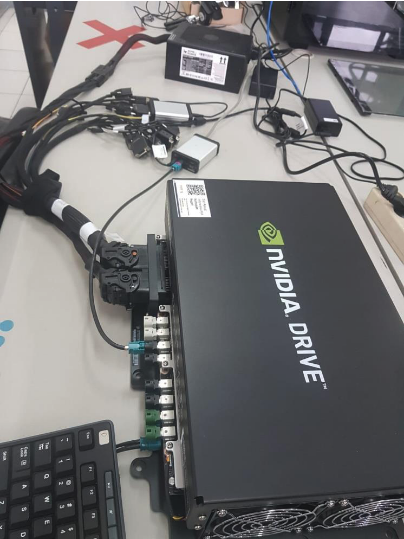
\includegraphics[height=0.5\textheight]{resources/chapter-2/pegasus.png}
        \caption{NVIDIA Pegasus \parencite{trilaksono_laporanRispro}}
    \end{center}
\end{figure}

Mengutip dari \parencite{oh_2017}, NVIDIA Pegasus adalah komputer yang
mendukung pengemudian \textit{autonomous} secara penuh. Artinya, NVIDIA Pegasus
dapat digunakan untuk membuat sebuah kendaraan bermotor menjadi
\textit{autonomous vehcile} jika sensor dan algoritma yang digunakan tepat.

NVIDIA Pegasus menggunakan 2 GPU dengan arsitektur post-Volta dan 2 SoC NVIDIA
Xavier. Kombinasi CPU dan GPU ini dapat menghasilkan 320 TOPS (\textit{trillion
    operations/second}) untuk komputasi intelegensi buatan. Untuk koneksi I/O,
NVIDIA Pegasus mendukung sampai dengan 16 kamera (6 di antaranya adalah lidar).

% TODO: Jelasin/masukin hubungannya dengan CARLA dan jelasin juga kalo NVIDIA
% Pegasus ini komputer biasa yang bisa menggunakan berbagai OS (buat transisi ke
% rosbridge)

\section{Metode Komunikasi antara Simulator CARLA dan NVI\-DI\-A Pegasus}

Pada keadaan yang ada, komunikasi antara simulator CARLA dengan NVIDIA Pegasus
menggunakan perantara \textit{web service} yang berbasis HTTP. Penggunaan HTTP
pada \textit{web service} menjadi \textit{bottleneck}/penghambat kinerja
terbesar sistem simulasi. Ketika dilakukan secara SILS (\textit{software in the
    loop simulation} tanpa NVIDIA Pegasus) didapatkan kinerja 4000 transaksi per
detik, sedangkan ketika NVIDIA Pegasus ditambahkan ke sistem (menjadi HILS,
\textit{hardware in the loop simulation}) didapatkan 100--110 transaksi per
detik \parencite{trilaksono_laporanRispro}. Oleh karena itu, dibutuhkan protokol
atau metode komunikasi lain yang dapat meningkatkan kinerja jalur komunikasi.
Selain itu, jalur komunikasi yang digunakan harus dapat mengirimkan pesan berupa
teks \textit{string}, larik angka, atau data \textit{binary} (misalnya gambar).

\begin{figure}
    \begin{center}
        \includegraphics[width=1.0\textwidth]{resources/chapter-2/komunikasi
            data pada simulasi.png}
        \caption{arsitektur komunikasi data pada HILS
            \parencite{trilaksono_laporanRispro}}
    \end{center}
\end{figure}

Beberapa alternatif metode/protokol jalur komunikasi dapat digunakan untuk
meng\-hu\-bung\-kan sistem ini akan dibahas pada subbab ini. Protokol atau
metode tersebut adalah rosbridge, RPC, dan \textit{messaging system}.

\subsection{Rosbridge}

Rosbridge adalah protokol komunikasi yang menambahkan antarmuka pada komputer
dengan sistem operasi ROS. Antarmuka yang ditambahkan membuat komputer dapat
\textit{publish} dan \textit{subscribe} ke topik ROS dalam format JSON. Selain
itu, antarmuka tersebut memungkinkan memanggil \textit{service} ROS di antara
hal-hal lainnya.

Spesifikasi lengkap untuk rosbridge tertuang di proyek \parencite{ros_bridge}.
Pada subbab ini, spesifikasi rosbridge akan dijelaskan secara singkat.

Secara arsitektur, protokol rosbridge menggunakan protokol WebSocket untuk
la\-pi\-san transpornya. Protokol WebSocket sendiri berjalan di atas protokol TCP
yang artinya protokol rosbridge menjamin data akan sampai dengan urutan yang
benar.

Protokol rosbridge menggunakan format JSON untuk pesannya. Pesan yang valid
harus mengandung \textit{field} \texttt{"op"}. \textit{Field} tersebut digunakan
untuk menentukan jenis pesan. Pesan juga dapat mengandung \textit{field}
\texttt{"id"} yang digunakan sebagai penanda transaksi atau keterhubungan antara
beberapa pesan. Selain kedua \textit{field} tersebut, pesan rosbridge juga dapat
mengandung \textit{field} lainnya tergantung jenis \texttt{"op"}.

\begin{lstlisting}[language=JSON, caption=contoh pesan valid pada lapisan
transpor rosbridge]
{
    "op": "fragment"
}
\end{lstlisting}

Jenis pesan yang dapat dikirim dapat dibagi menjadi 3 kategori.
Kategori-kategori tersebut akan diuraikan sebagai berikut.
\begin{enumerate}
    \item Pesan kompresi atau transformasi dengan kode \texttt{op}:
          \begin{itemize}
              \item \texttt{fragment} untuk pesan yang terpecah-pecah, atau
              \item \texttt{png} untuk pesan yang berupa berkas PNG.
          \end{itemize}
    \item Pesan status rosbridge:
          \begin{itemize}
              \item \texttt{set\_status\_level} untuk mengatur tingkat pelaporan
                    rosbridge, atau
              \item \texttt{status} untuk pesan status.
          \end{itemize}
    \item Pesan operasi:
          \begin{itemize}
              \item \texttt{advertise} untuk menandakan pengirim sedang
                    mempublikasikan suatu topik,
              \item \texttt{unadvertise} untuk menandakan pengirim berhenti
                    mempublikasikan suatu topik,
              \item \texttt{publish} untuk pesan ROS yang dipublikasikan ke
                    suatu topik,
              \item \texttt{subscribe} untuk meminta ``berlangganan'' ke suatu
                    topik,
              \item \texttt{unsubscribe} untuk meminta berhenti ``berlangganan'',
              \item \texttt{call\_service} untuk memanggil suatu layanan,
              \item \texttt{advertise\_service} untuk menandakan pengirim
                    sedang mem\-pu\-bli\-ka\-si\-kan suatu layanan, \item
                    \texttt{unadvertise\_service} untuk menandakan pengirim
                    berhenti mempublikasikan suatu layanan,
              \item \texttt{service\_request} untuk \textit{request}/permintaan
                    ke suatu layanan, atau \item \texttt{service\_response} untuk
                    hasil/balasan permintaan ke suatu layanan.
          \end{itemize}
\end{enumerate}

Pesan yang dikirim melalui protokol rosbridge dapat di-\textit{encode} dengan 3
format. Format pertama adalah \textit{raw} JSON. Dalam format ini, pesan yang
dikirim akan berupa \textit{string} biasa. Selain itu, pesan yang dikirim juga
dapat dikompresi dengan format CBOR (\textit{concise binary object
    representation}) atau CBOR-\textit{raw}. Pesan dalam format CBOR akan
berbentuk pesan \textit{binary}. Sehingga pesan harus didekompresi oleh
penerima untuk mendapatkan pesan aslinya.

Perbedaan antara CBOR dengan CBOR-\textit{raw} adalah format pesannya. Pada
CBOR-\textit{raw}, pesan dikirim dalam format serialisasi ROS. Format
serialisasi ROS digunakan untuk mengirimkan data antar-ROS \textit{node} dan
pada berkas \texttt{bag}\footnote{Format berkas yang digunakan untuk menyimpan
    data pada mesin ROS.}. Keuntungan menggunakan CBOR-\textit{raw} adalah
peningkatan kinerja jika \textit{parsing} hanya sebagian pesan, aplikasi dapat
membaca berkas \texttt{bag}, atau \textit{parsing} pesan ingin dilakukan
seterlambat mungkin atau secara paralel.

\subsection{RPC}

RPC, atau \textit{remote procedure call}, secara teknis bukanlah protokol,
melainkan sebuah mekanisme untuk menyusun sistem terdistribusi yang
berkomunikasi dengan pola \textit{request/reply}
\parencite{larry_computerNetwork}. RPC memberikan abstraksi kepada pengembang
berupa pemanggilan fungsi secara lokal maupun \textit{remote}, di permukaannya,
memiliki perilaku yang sama. Pemanggilan fungsi \textit{remote} artinya
implementasi fungsi berada di komputer lain di dalam jaringan.

Ketika menggunakan RPC, pengembang tidak perlu tahu pemanggilan sebuah fung\-si
dilakukan secara lokal atau \textit{remote}; pengembang hanya tahu pemanggilan
fungsi tersebut akan menghasilkan suatu nilai baru dan dapat (tidak
selalu\footnote{Beberapa implementasi RPC mendukung pemanggilan
    \textit{asynchronous} yang tidak harus memberikan sebuah \textit{return}
    (misalnya Apache Thrift dengan kata kunci \texttt{async}/\texttt{oneway}
    \parencite{agarwal_thrift}).})
membuat program \textit{blocking} (menunggu) sampai nilai baru tersebut
didapatkan.

Abstraksi RPC ``diberikan'' oleh 2 komponen utama pada RPC. Komponen pertama
adalah protokol yang mengurusi pengiriman pesan antara \textit{server/producer}
dan \textit{client/consumer}. Kedua, bahasa pemrograman dan \textit{compiler}
yang dapat membungkus pemanggilan fungsi \textit{remote} menjadi pesan
\textit{request} dan mentranslasikan pesan \textit{request} menjadi pemanggilan
ke fungsi lokal (begitu juga untuk \textit{return} dari pemanggilan fungsi
\textit{remote}).

Secara arsitektur, RPC bisa dibangun di atas protokol TCP sehingga pembuat
implementasi RPC tidak perlu memikirkan keandalan (\textit{reliability})
pengiriman pesan pada implementasinya. Akan tetapi, RPC juga bisa dibangun di
atas protokol UDP atau IP lalu ditambahkan/dibuat lapisan keandalannya sendiri.

Implementasi RPC yang akan dibahas pada subbab ini adalah Apache Thrift.
Apa\-che Thrift juga merupakan implementasi RPC yang akan digunakan untuk
membangun jalur komunikasi antara server NVIDIA Pegasus dengan server simulator
CARLA. Apache Thrift dipilih karena kemampuannya mengirimkan pesan dalam format
\textit{binary}. Selain itu, karena kinerja Apache Thrift lebih baik
dibandingkan dengan HTTP dan implementasi RPC oleh Google, gRPC
\parencite{abernethy_buildingHighPerformanceMSThrift}.

\subsubsection{Apache Thrift}

Apache Thrift adalah sebuah implementasi RPC dalam bentuk \textit{framework}
yang diciptakan oleh Facebook, Inc. (sekarang Meta Platforms, Inc.) lalu
disumbangkan ke Apache Software Foundation. Tujuan utama dari pembuatan Apache
Thrift adalah sebuah jembatan antar-bahasa pemrograman yang memiliki kinerja
tinggi \parencite{agarwal_thrift} sehingga Apache Thrift dapat digunakan lintas
bahasa pemrograman.

Apache Thrift memiliki beberapa abstraksi yang memudahkan pengembang untuk
menggunakan RPC. Abstraksi-abstraksi tersebut adalah sistem tipe, protokol,
transpor, pemberian versi, dan prosesor.

Sistem tipe pada Apache Thrift bertindak sebagai \textit{common language}
antar-bahasa pemrograman. Dengan adanya sistem tipe ini, sebuah definisi untuk
Apache Thrift dapat digunakan untuk banyak bahasa tanpa mengharuskan pemrogram
menulis tipe data buatan atau kode serialisasi sendiri. Tipe-tipe yang ada pada
sistem tipe Apache Thrift adalah \parencite{agarwal_thrift}
\begin{itemize}
    \item tipe dasar: \texttt{bool}, \texttt{byte}, \texttt{i16},
          \texttt{i32}, \texttt{i64}, \texttt{double}, dan \texttt{string},
    \item tipe struktur data (``\textit{struct}''): tipe komposit yang setara
          dengan kelas data pada pemrograman berorientasi objek atau \texttt{struct}
          pada C,
    \item \textit{container}: kumpulan data dan terdiri atas
          \begin{itemize}
              \item \texttt{list<type>}: daftar terurut dari beberapa elemen
                    dengan tipe \texttt{type},
              \item \texttt{set<type>}: himpunan elemen dengan tipe
                    \texttt{type} yang tidak terurut, dan
              \item \texttt{map<type1, type2>}: \textit{map} dengan \textit{key}
                    unik bertipe \texttt{type1} yang di\-pe\-ta\-kan tepat ke 1
                    \textit{value} bertipe \texttt{type2},
          \end{itemize}
    \item \textit{exception}: galat dan pendefinisiannya sama dengan
          \textit{struct}, dan
    \item layanan (``\textit{service}''): akan menciptakan \textit{interface}
          (atau padanannya) di bahasa target.
\end{itemize}

Data-data yang ingin digunakan pada sistem dan sesuai dengan sistem tipe Thrift
dapat dituliskan pada Thrift IDL (\textit{interface definition language}).
Thrift IDL memungkinkan pendefinisian struktur-struktur data tanpa harus
menuliskan informasi cara mentransportasikan data dengan aman. Struktur data
yang dapat didefinisikan pada Thrift IDL adalah \textit{struct}, \textit{enum},
konstanta (``\textit{const}''), alias tipe (\texttt{typedef} di C), \textit{union}
(\texttt{union} di C), dan \textit{exception}. IDL akan digunakan pembangkit
kode Thrift untuk membangkitkan kode pada bahasa target sehingga dapat
menggunakan layanan dan struktur data pada IDL.

Abstraksi transpor pada Apache Thrift membangkitkan kode yang dapat
di\-gu\-na\-kan untuk transpor data. Dengan adanya abstraksi ini, antarmuka
aliran data dapat dengan mudah diubah-ubah. Kode yang dibangkitkan Thrift juga
tidak peduli dengan sumber data sehingga dengan adanya abstraksi ini pengguna
Thrift dapat memilih media transpor data dengan bebas dan mudah.
\textit{Interface} untuk abstraksi transpor adalah \texttt{TTransport}.

Abstraksi protokol memisahkan struktur data dari representasi yang digunakan
untuk transpor. Dengan adanya abstraksi protokol, pengguna Thrift tidak perlu
me\-mi\-kir\-kan cara \textit{encoding} dan \textit{decoding} data yang ingin dikirim
melalui abstraksi transpor. \textit{Interface} untuk abstraksi protokol adalah
\texttt{TProtocol}.

Abstraksi \textit{versioning} bertujuan memudahkan pembaharuan layanan dan
struktur data. Abstraksi ini dicapai dengan penambahan sebuah nomor
\textit{identifier} sebelum \textit{field} pada \textit{struct} dan
\textit{exception} serta pada argumen untuk metode-metode layanan.

Abstraksi prosesor adalah abstraksi yang untuk memproses data dan melakukan RPC.
Abstraksi prosesor menggunakan \textit{interface} \texttt{TProcessor} dan
memiliki sebuah metode \texttt{process} untuk menangani pemanggilan RPC.

Thrift juga menyediakan sebuah \textit{interface} \texttt{TServer}.
\texttt{TServer} bertanggung jawab atas pengurusan koneksi, \textit{threading},
dll. sedangkan \texttt{TProcessor} bertanggung jawab atas penanganan pemanggilan
RPC. Salah satu pekerjaan \texttt{TServer} adalah memanggil metode
\texttt{process} pada \texttt{TProcessor}.

\textit{Interface} \texttt{TServer} dan \texttt{TProcessor} akan dibangkitkan
pada server/produsen. Se\-dang\-kan pada klien/konsumen akan dibangkitkan
implementasi untuk \textit{interface}/la\-ya\-nan pada IDL, disebut
\textit{client}. Implementasi pada klien memanfaatkan 2 buah \texttt{TProtocol}
untuk melakukan proses I/O.

\begin{figure}
    \begin{center}
        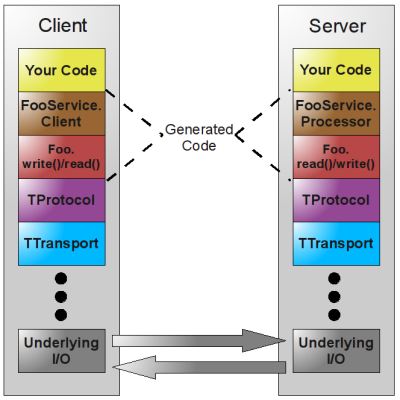
\includegraphics[width=0.25\textheight]{resources/chapter-2/thrift-arch.png}
        \caption{arsitektur Apache Thrift \parencite{prunicki_thrift}}
    \end{center}
\end{figure}

Secara bawaan, Apache Thrift mendukung beberapa transpor, protokol, dan server
\parencite{prunicki_thrift}. Dukungan-dukungan tersebut adalah
\begin{itemize}
    \item transpor (implementasi \texttt{TTransport}):
          \begin{itemize}
              \item \texttt{TSim\-ple\-FileTrans\-port}: menggunakan berkas,
              \item \texttt{TMe\-mo\-ry\-Trans\-port}: menggunakan memori,
              \item \texttt{T\-Sock\-et}: \textit{socket blocking},
              \item \texttt{TFramed\-Trans\-port}: pada server
                    \textit{nonblocking}, dan
              \item \texttt{T\-Z\-lib\-Trans\-port}: Melakukan kompresi dengan
                    zlib dan harus digunakan dengan trans\-por lain,
          \end{itemize}
    \item protokol (implementasi \texttt{TProtocol}):
          \begin{itemize}
              \item \texttt{TBinaryProtocol}: pesan dikirim dalam format
                    \textit{binary},
              \item \texttt{TCompactProtocol}: \texttt{TBinaryProtocol} yang
                    lebih \textit{compact},
              \item \texttt{TDenseProtocol}: \texttt{TCompactProtocol} yang
                    di\-hi\-lang\-kan \textit{me\-ta\-da\-ta}-nya, lalu ditambahkan
                    lagi oleh penerima,
              \item \texttt{TJsonProtocol}: pesan dikirim dalam format JSON,
              \item \texttt{TSimpleJsonProtocol}: \texttt{TJsonProtocol} tanpa
                    \textit{metadata}, cocok untuk bahasa \textit{scripting}, dan
              \item \texttt{TDebugProtocol}: format paling mudah dibaca manusia,
          \end{itemize}
    \item server (implementasi \texttt{TServer}):
          \begin{itemize}
              \item \texttt{TSimpleServer}: server \textit{single-threaded},
              \item \texttt{TThreadPoolServer}: server \textit{multi-threaded}
                    dengan \textit{blocking} I/O, dan
              \item \texttt{TNonBlockingServer}: server \textit{multi-threaded}
                    dengan \textit{non-blocking} I/O dan harus menggunakan
                    \texttt{TFramedTransport}.
          \end{itemize}
\end{itemize}

\subsection{\textit{Messaging System}}

\subsubsection{ZeroMQ}

\section{Penelitian Terkait}
\blindtext